%!TEX root = main.tex
\section{Details in Section~\ref{sec:symbolic}}\label{app-sym}

\subsection{Proof of the first result in Proposition~\ref{prop-2nsa}}

Let $\Aut = (\Upsilon, \EndLeft, \EndRight, \controls, q_0, \finals, \transrel)$ be a \SSA. We show how to construct an equivalent \SA{} $\Aut' =  (\Upsilon, \controls', q'_0, \finals', \transrel')$.
W.l.o.g., we assume that for each transition $(q, \psi, dir, q') \in \transrel$, we have $dir \in \{\Left,\Right\}$. Every \SSA{} can be turned into one satisfying the assumption as follows: Replace each transition $(q, \psi, \Stay, q') \in \transrel$ with the following three transitions $(q, \psi, \Right, q'')$, $(q'', \ltrue, \Left, q')$, and $(q'', \EndRight, \Left, q')$, where $q''$ is a fresh state.

The proof is an adaptation of the  construction of nondeterministic one-way automata from two-way nondeterministic finite state automata based on the idea of crossing sequences (cf. e.g. \cite{HU79}). Since \SSA{}s replace the letters in \FFA{}s with unary predicates, the main technical challenge is to deal with these guards in a proper way.

We first use an example to illustrate the idea of crossing sequences: Suppose $w = \EndLeft d_1 d_2 d_3 d_4 d_5\EndRight$, and an accepting run of $\Aut$ on $w$ uses the following sequence of transitions 
\[
\begin{array}{l}
(q_0, \EndLeft, \Right, q_1), (q_1, \psi_1, \Right, q_1), (q_1, \psi_2, \Left, q_2), (q_2, \psi_3, \Right, q_0), (q_0, \psi_4, \Right, q_1), \\
(q_1, \psi_1, \Right, q_1), (q_1, \psi_1, \Right, q_1), (q_1, \psi_2, \Left, q_2), (q_2, \psi_3, \Right, q_0), (q_0, \psi_4, \Right, q_1),
\end{array}
\] 
with $q_1 \in \finals$.
The run is illustrated in Figure~\ref{fig-2sa-sa}. A \emph{crossing sequence} of the run is a sequence of states in the boundary of two tape cells, e.g. the sequence $q_1, q_2, q_0$ in the boundary of $d_1$ and $d_2$. Note that for technical convenience, the states of the run are put in a \emph{special} manner that whenever a left-transition $(q, \psi, \Left, q')$ is taken, $q'$ is put just below $q$, thus in the \emph{same} crossing sequence as $q$, instead of putting $q'$ in the crossing sequence on-position to the left. Therefore, 
\emph{the target state of each left-transition is put in the position right-adjacent to the actual position of the reading head}.
For instance, in Figure~\ref{fig-2sa-sa}, when the transition $(q_1, \psi_2, \Left, q_2)$ is taken, $q_2$ is put just below $q_1$. Compared to the crossing sequences for 2FAs, in Figure~\ref{fig-2sa-sa}, we also include the guards of transitions. 

\begin{figure}[htbp]
\begin{center}
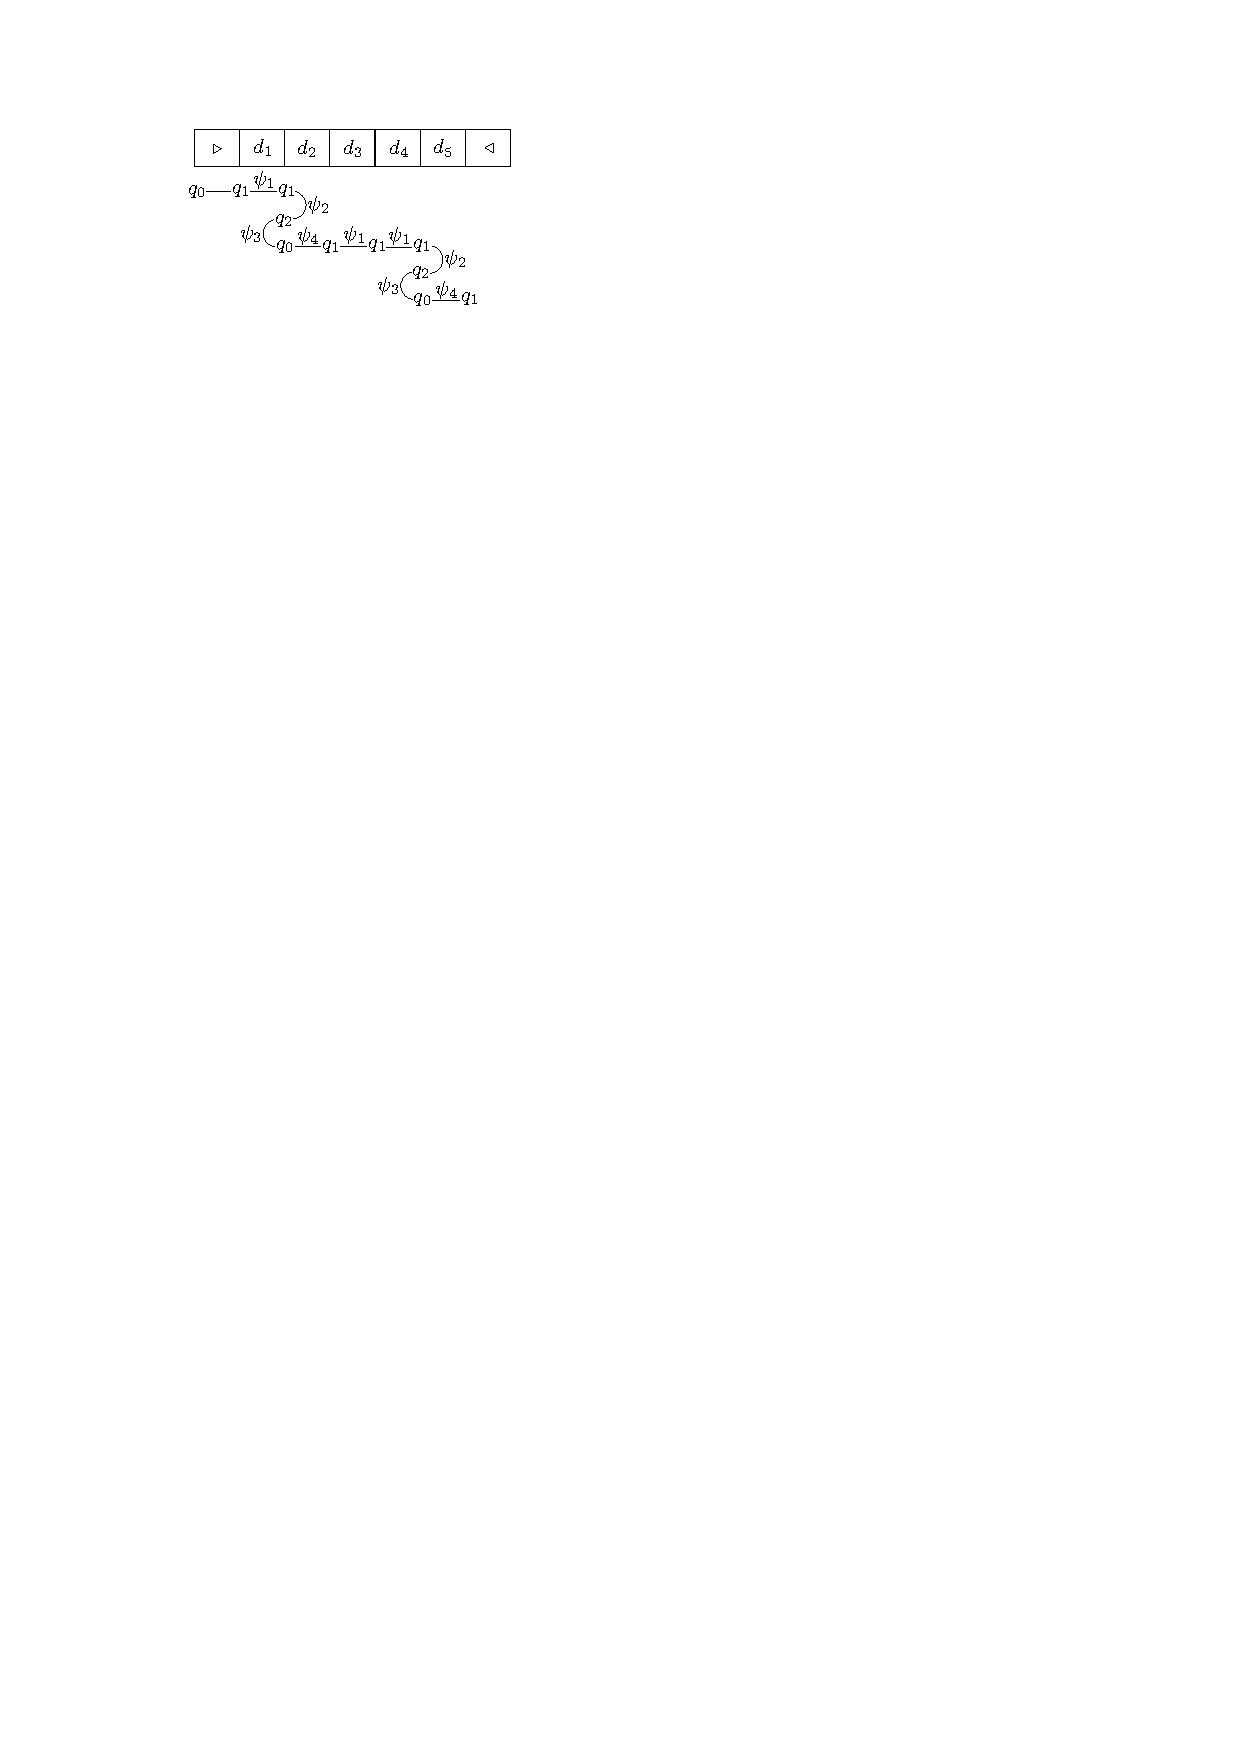
\includegraphics{2sa-sa-exmp.pdf}
\end{center}
\caption{Accepting runs of $\Aut$: An example}\label{fig-2sa-sa}
\end{figure}

In order to deal with the guards in transitions, we adapt the crossing sequences of the \SSA{} $\Aut$  as follows: a crossing sequence of $\Aut$ is a sequence of transitions of odd lengths, such that  the source states of the transitions in the even (resp. odd) positions are mutually distinct. Let $S_\transrel$ denote the set of such sequences of transitions.


\newcommand\lmatch{\mathsf{LeftMatch}}
\newcommand\rmatch{\mathsf{RightMatch}}

In order to construct the set of transitions of $\Aut'$, we shall define two \emph{partial} functions $\lmatch(\rho_1, \rho_2)$ and $\rmatch(\rho_1, \rho_2)$ for $\rho_1, \rho_2 \in S_\transrel$. 
The intention of $\lmatch(\rho_1, \rho_2)$ and $\lmatch(\rho_1, \rho_2)$ is explained as follows.
\begin{itemize}
\item The intention of $\lmatch(\rho_1, \rho_2)$: $\rho_1$ and $\rho_2$ are the crossing sequences to the left resp. right of some position $i$ holding a data value $d$, and initially, we reach the source state of the first transition of $\rho_2$ by a \emph{left-transition} (thus after this transition, the reading head is in the position $i$\footnote{Recall that the target state of each left-transition is put in the position right-adjacent to the actual position of the reading head.}).
%
\item The intention of $\rmatch(\rho_1, \rho_2)$:  $\rho_1$ and $\rho_2$ are the crossing sequences to the left resp. right of some position $i$ holding a data value $d$, and initially, we reach the source state of the first transition of $\rho_1$, say $p_1$, by a \emph{right-transition} (thus after this transition, the reading head is in the position $i$).
\end{itemize}
%
Formally, the domain of $\lmatch$ (resp. $\rmatch$) is defined inductively as follows, where in each case below, the return value is also specified.  \\
Let $\rho_1, \rho_2 \in S_\transrel$. Then $\lmatch(\rho_1, \rho_2)$ is defined iff one of the following constraints holds.
\begin{itemize}
\item Case $\rho_1 = \varepsilon$, $\rho_2 = \varepsilon$: $\lmatch(\rho_1, \rho_2) = \ltrue$.
%
\item Case $\rho_1 =  \tau_{1,1}, \ldots, \tau_{1,k}$ with $k \ge 1$, $\rho_2 = \tau_{2,1}, \ldots, \tau_{2,l}$ with $l \ge 1$, $\tau_{2,1} = (q_1, \psi_{2,1}, \Left, p_1)$, $p_1$ is the source state of $\tau_{1,1}$, and $\rmatch(\rho'_1, \rho'_2)$ is defined:  
$$\lmatch(\rho_1, \rho_2) = \psi_{2,1} \wedge \rmatch(\rho'_1, \rho'_2),$$ 
where $\rho'_1 = \tau_{1,2}, \ldots, \tau_{1,k}$ and $\rho'_2 = \tau_{2,2}, \ldots, \tau_{2,l}$.
%
\item Case $\rho_1 =  \tau_{1,1}, \ldots, \tau_{1,k}$ with $k \ge 1$, $\rho_2 = \tau_{2,1}, \ldots, \tau_{2,l}$ with $l \ge 1$, $\tau_{2,1} = (q_1, \psi_{2,1}, \Right, q_2)$, $q_2$ is the source state of $\tau_{2,2}$, and $\lmatch(\rho_1, \rho'_2)$ is defined:  
$$\lmatch(\rho_1, \rho_2) = \psi_{2,1} \wedge \lmatch(\rho_1, \rho'_2),$$ 
where $\rho'_2 = \tau_{2,3}, \ldots, \tau_{2,l}$.
%
\end{itemize} 
%
Symmetrically, $\rmatch(\rho_1, \rho_2)$ is defined iff one of the following constraints holds.
\begin{itemize}
\item Case $\rho_1 = \varepsilon$, $\rho_2 = \varepsilon$: $\rmatch(\rho_1, \rho_2) = \ltrue$.

\item Case $\rho_1 =  \tau_{1,1}, \ldots, \tau_{1,k}$ with $k \ge 1$, $\rho_2 = \tau_{2,1}, \ldots, \tau_{2,l}$ with $l \ge 1$, $\tau_{1,1} = (p_1, \psi_{1,1}, \Right, q_1)$, $q_1$ is the source state of $\tau_{2,1}$, and $\lmatch(\rho'_{1}, \rho'_2)$ is defined:  
$$\rmatch(\rho_1, \rho_2) =\psi_{1,1} \wedge \lmatch(\rho'_{1}, \rho'_2),$$ 
where $\rho'_1 = \tau_{1, 2},\ldots, \tau_{1,k}$, and $\rho'_2 = \tau_{2,2}, \ldots, \tau_{2,l}$.
%
\item Case $\rho_1 =  \tau_{1,1}, \ldots, \tau_{1,k}$ with $k \ge 1$, $\rho_2 = \tau_{2,1}, \ldots, \tau_{2,l}$ with $l \ge 1$, $\tau_{1,1} = (p_1, \psi_{1,1}, \Left, p_2)$, $p_2$ is the source state of $\tau_{1,2}$, and $\rmatch(\rho'_1, \rho_2)$ is defined:  
$$\rmatch(\rho_1, \rho_2) = \psi_{1,1} \wedge \rmatch(\rho'_1, \rho_2),$$ 
where $\rho'_1 = \tau_{1,3}, \ldots, \tau_{1,k}$.
%
\end{itemize}

We are ready to construct the \SA{} $\Aut' =  (\Upsilon, \controls', q'_0, \finals', \transrel')$, where
\begin{itemize}
\item $\controls' = S_\transrel \cup \{q'_0\}$, where $q'_0$ is a fresh state not in $S_\transrel$,
%
\item $\finals'$ comprises the set of elements $\rho \in S_\transrel$ satisfying that: suppose $\rho = \tau_1, \ldots, \tau_{2n+1}$, for each $i \in [n+1]$, $\tau_{2i-1} = (p_{2i-1}, \EndRight, \Left, q_{2i-1})$, and for each $i \in [n]$, $\tau_{2i} = (p_{2i}, \psi_{2i}, dir_{2i}, q_{2i})$, then $q_{2n+1} \in F$, moreover, for each $i \in [n]$, $q_{2i-1} = p_{2i}$,  
%
\item $\transrel'$ comprises the following transitions: 
%
\begin{itemize}
%
\item for each $\rho, \rho' \in S_\transrel$ such that $\rmatch(\rho, \rho')$ is defined, we have $(\rho, \rmatch(\rho, \rho'), \rho') \in \transrel'$,
%
\item  
%the transitions out of $q'_0$ are defined as follows:
%
for each $\rho \in I'$ and $\rho' \in S_\transrel$ such that $\rmatch(\rho, \rho')$ is defined, we have $(q'_0, \rmatch(\rho, \rho'), \rho') \in \transrel'$, where 
$I'$ comprises $\rho'' \in S_\transrel$ satisfying the following constraints: $\rho'' = \tau_1, \ldots, \tau_{2n+1}$,  for each $i \in [n+1]$, $\tau_{2i-1} = (p_{2i-1}, \psi_{2i-1}, dir_{2i-1}, q_{2i-1})$, for each $i \in [n]$, $\tau_{2i} = (p_{2i}, \EndLeft, \Right, q_{2i})$, moreover, $(q_0, \EndLeft, \Right, p_1) \in \transrel$, and for each $i \in [n]$, $q_{2i} = p_{2i+1}$. 
\end{itemize}
%
\end{itemize}

Since $S_\transrel$ contains at most $(\numtrans(\Aut))^{2|\controls|-1} \le (\numtrans(\Aut))^{2\numtrans(\Aut)}$ elements, we conclude that 
$$
\begin{array}{l c l}
\numtrans(\Aut') \le ((\numtrans(\Aut))^{2\numtrans(\Aut)})^2  & = & (\numtrans(\Aut))^{4\numtrans(\Aut)} 
 \approx    2^{O\left(\numtrans(\Aut) \log \numtrans(\Aut)\right)}
\end{array}
$$ 
and 
$$
\begin{array}{l c l}
\sizetrans(\Aut') \le 2(2|\controls|-1)\sizetrans(\Aut)  & \le & 4 \numtrans(\Aut) \sizetrans(\Aut) 
\approx   O( \numtrans(\Aut) \sizetrans(\Aut)).
\end{array}
$$


\subsection{Proof of Lemma~\ref{lem-spt}}
